\chapter{La suma de convoluci\'{o}n}

\section{Deducci\'{o}n de la f\'{o}rmula}

A continuaci\'{o}n calculamos la salida $y[n]$ de un sistema lineal  para una entrada arbitraria $x[n]$. 
Para poder hacerlo, usamos pulsos desplazados en el tiempo $\delta[n-n_{0}]$ 
donde $n_{0}$ es un instante de tiempo.

\subsection{Representaci\'{o}n de se\~{n}ales en t\'{e}rminos de
  impulsos}

\begin{enumerate}

\item Consideremos una secuencia $x\left[ n\right]$, (ver
  Fig.(\ref{convoneeps})).  Por la propiedad del muestreo podemos
  escribir
  \begin{eqnarray}
    x[-2]\delta \left[ n+2\right]   &=&     \left\{ \begin{array}{ll}
        x[-2],  & n=-2,                 \\ 
        0,      & n\neq -2,
      \end{array}
    \right.                                         \\
    x[-1]\delta \left[ n+1\right]   &=&     \left\{ \begin{array}{ll}
        x[-1],  & n=-1,                 \\ 
        0,      & n\neq -1,
      \end{array}
    \right.                                                 \\
    x[0]\delta \left[ n\right]      &=&     \left\{ \begin{array}{ll}
        x[0],   & n=0,                  \\ 
        0,      & n\neq 0,
      \end{array}
    \right.                                                 \\
    x[1]\delta \left[ n-1\right]    &=&     \left\{ \begin{array}{ll}
        x[1],   & n=1,                  \\ 
        0,      & n\neq 1,
      \end{array}
    \right.                                                 \\
    x[2]\delta \left[ n-2\right]   &=&     \left\{ \begin{array}{ll}
        x[2],   & n=2,                  \\ 
        0,      & n\neq 2,
      \end{array}
    \right.
  \end{eqnarray}
  y en general,
  \begin{equation}
    x[k]\delta \left[ n-k\right] =  \left\{ \begin{array}{ll}
        x[k],   & n=k,          \\ 
        0,      & n\neq k.
      \end{array}
    \right.
  \end{equation}

\item Como podemos ver en la Fig.(\ref{repconvoneeps}), la suma de
  impulsos desplazados en el tiempo multiplicados por coeficientes
  adecuados equivalen a cualquier se\~{n}al arbitraria $x[n]$.
  \begin{figure}
    \centering
    \includegraphics[width=3in]{./graphics/convone.eps}
    \caption{Una se\~{n}al como suma de impulsos desplazados en el
      tiempo multiplicados por coeficientes adecuados. Los impulsos
      desplazados $\delta[n-k]$ se representan $d[n-k]$.  S\'{o}lo se
      muestran tres impulsos por razones de espacio.}
    \label{repconvoneeps}
  \end{figure}
        
\item En efecto, agregando m\'{a}s impulsos desplazados y
  multiplicados adecuadamente podemos obtener una expresi\'{o}n que se
  puede escribir en forma general
  \begin{equation}
    x\left[ n\right] =
    \sum_{k=-\infty }^{\infty }x\left[ k\right] \delta \left[n-k\right] .  \label{cduna.5}
  \end{equation}

\item La Ec. (\ref{cduna.5}) corresponde a la representaci\'{o}n de una
  secuencia arbitraria $x[n]$ como
  \begin{itemize}
  \item una combinaci\'{o}n lineal de impulsos desplazados $\delta
    \left[ n-k\right]$,
                        
  \item donde los coeficientes de la combinaci\'{o}n lineal son los
    valores $x[k]$.
  \end{itemize}
                
\item Cada impulso desplazado $\delta \left[ n-k\right] $ act\'{u}a
  como selector: suponga que elegimos un valor $n=n_{0}$ y entonces
  tenemos que
  \begin{equation}
    x\left[ n_{0}\right] =
    \sum_{k=-\infty }^{\infty }x\left[ k\right] \delta \left[ n_{0}-k\right] .  
    \label{cddos.5}
  \end{equation}
                
\item Recordemos la definici\'{o}n de impulso
  \begin{equation}
    \delta \left[ n\right] =\left\{ 
      \begin{array}{cc}
        1, & n=0, \\ 
        0, & n\neq 0.
      \end{array}
    \right.
  \end{equation}
  El impulso ``vale'' $1$ cuando el \'{\i}ndice $n$ (lo que aparece
  entre corchetes) vale $0$. Note que en la ec. (\ref{cddos.5}) s\'{o}lo
  uno de los infinitos impulsos tiene un \'{\i}ndice nulo,
  espec\'{\i}ficamente
  \begin{equation}
    n_{0}-k=0.
  \end{equation}
  Entonces, de todos los infinitos t\'{e}rminos s\'{o}lo uno es no
  nulo ($k=n_{0})$.  As\'{\i} obtenemos la igualdad
  \begin{equation}
    x\left[ n_{0}\right] =x\left[ n_{0}\right] .
  \end{equation}

\item La utilidad de la ecuaci\'{o}n (\ref{cduna.5}) es que expresa una
  secuencia
  \begin{equation}
    ...x[-3], \, x[-2], \, x[-1], \, x[0], \, x[1], \, x[2], \, x[3]...
  \end{equation}
  como una sumatoria.

\end{enumerate}

\subsection{La respuesta al impulso y la suma de convoluci\'{o}n}

\begin{enumerate}

\item Sea $h_{k}\left[ n\right] = h\left[ n-k\right] $ la respuesta de
  un sistema lineal $S$ al impulso unitario desplazado $\delta \left[
    n-k\right]$,
  \begin{equation}
    \begin{array}{c}
      ... \\ 
      \delta \left[ n+1\right] 
      \begin{array}{c}
        S \\ 
        \rightarrow
      \end{array}
      h_{-1}\left[ n\right] , \\ 
      \delta \left[ n\right] 
      \begin{array}{c}
        S \\ 
        \rightarrow
      \end{array}
      h_{0}\left[ n\right] , \\ 
      \delta \left[ n-1\right] 
      \begin{array}{c}
        S \\ 
        \rightarrow
      \end{array}
      h_{1}\left[ n\right] , \\ 
      ... \\ 
      \delta \left[ n-k\right] 
      \begin{array}{c}
        S \\ 
        \rightarrow
      \end{array}
      h_{k}\left[ n\right] .
    \end{array}
  \end{equation}
  Vea la Fig.(\ref{convtwooneeps}).
  \begin{figure}
    \centering
    \includegraphics[width=3in]{./graphics/convtwoone.eps}
    \caption{Las respuestas de un sistema lineal frente a impulsos
      desplazados en el tiempo. Los gr\'{a}ficos de la columna
      izquierda representan las entradas, y los de la columna derecha
      las salidas.}
    \label{convtwooneeps}
  \end{figure}

\item Como el sistema $S$ es lineal, podemos multiplicar a ambos lados
  por constantes y obtenemos
  \begin{equation}
    \begin{array}{c}
      ... \\ 
      x\left[ -1\right] \delta \left[ n+1\right] 
      \begin{array}{c}
        S \\ 
        \rightarrow
      \end{array}
      x\left[ -1\right] h_{-1}\left[ n\right] , \\ 
      x\left[ 0\right] \delta \left[ n\right] 
      \begin{array}{c}
        S \\ 
        \rightarrow
      \end{array}
      x\left[ 0\right] h_{0}\left[ n\right] , \\ 
      x\left[ 1\right] \delta \left[ n-1\right] 
      \begin{array}{c}
        S \\ 
        \rightarrow
      \end{array}
      x\left[ 1\right] h_{1}\left[ n\right] , \\ 
      ... \\ 
      x\left[ k\right] \delta \left[ n-k\right] 
      \begin{array}{c}
        S \\ 
        \rightarrow
      \end{array}
      x\left[ k\right] h_{k}\left[ n\right] .
    \end{array}
  \end{equation}
  Como el sistema es lineal, podemos ``sumar'' las infinitas entradas
  y las infinitas salidas para obtener
  \begin{equation}
    x\left[ n\right] =\left( \sum_{k=-\infty }^{\infty }x\left[ k\right] \delta 
      \left[ n-k\right] \right) 
    \begin{array}{c}
      S \\ 
      \rightarrow
    \end{array}
    \left( \sum_{k=-\infty }^{\infty }x\left[ k\right] h_{k}\left[ n\right]
    \right) =y\left[ n\right] .     \label{convo}
  \end{equation}
  Vea la Fig.(\ref{convtwotwoeps}).

\begin{figure}
  \centering
  \includegraphics[width=3in]{./graphics/convtwotwo.eps}
  \caption{En la columna de la izquierda, desde la primera a la quinta
    fila vemos impulsos desplazados en el tiempo $\delta[n-k]$
    multiplicados por $x[k]$.  En la columna de la derecha, en las
    filas respectivas vemos las respuestas correspondientes.  En los
    subgr\'{a}ficos de la sexta fila, vemos la suma de los resultados
    parciales para obtener la se\~{n}al de entrada $x[n]$ (izquierda)
    y la salida correspondiente $y[n]$ (derecha)}
  \label{convtwotwoeps}
\end{figure}
Por el principio de superposici\'{o}n, $y\left[ n\right] $ es la
respuesta a la entrada $x\left[ n\right] $
\begin{equation}
  y\left[ n\right] =\sum_{-\infty }^{\infty }x\left[ k\right] h_{k}\left[ n\right]
\end{equation}

\item Si el sistema $S$ es invariante en el tiempo, entonces para
  cualquier valor de $k$ se cumple que
  \begin{equation}
    h_{k}\left[ n\right] =h_{0}\left[ n\right] .
  \end{equation}
  Por conveniencia notacional, definimos la respuesta al impulso de un
  sistema invariante en el tiempo
  \begin{equation}
    h\left[ n\right] =h_{0}\left[ n\right] ,
  \end{equation}
  o sea que $h\left[ n\right] $ es la salida de un sistema $S$ LIT
  cuando $\delta \left[ n\right] $ es la entrada. Entonces podemos
  escribir
  \begin{equation}
    h_{k}\left[ n\right] =  h\left[ n-k\right] ,
  \end{equation}
  y
  \begin{equation}
    y\left[ n\right] = \sum_{-\infty }^{\infty }x\left[ k\right] h\left[ n-k\right] .
  \end{equation}
  Esta es la suma de convoluci\'{o}n o superposici\'{o}n. La
  convoluci\'{o}n de dos se\~{n}ales se representa
  \begin{equation}
    y\left[ n\right] = x\left[ n\right] * h\left[ n\right] .
  \end{equation}

\end{enumerate}

\section{Ejemplos}

\subsection{Convolución con un impulso desplazado}

Supongamos un sistema con una respuesta al impulso $h[n] = \delta[n - n_{0}]$. Vamos a calcular su salida
para una entrada $x[n]$.

\begin{enumerate}
 \item Comenzamos escribiendo la suma de convolución
   \begin{equation}
    y\left[ n\right] = \sum_{-\infty }^{\infty }x\left[ k\right] h\left[ n-k\right] .
  \end{equation}
 \item Si $h[n] = \delta[n - n_{0}]$, entonces $h[n - k] = \delta[n - n_{0} - k]$.
 \item Reemplazando $h[n - k]$ en la suma de convolución resulta
   \begin{equation}
    y\left[ n\right] = \sum_{-\infty }^{\infty }x\left[ k\right] h\left[ n-k\right] =
    \sum_{-\infty }^{\infty }x\left[ k\right] \delta\left[ n- n_{0} -k\right].
  \end{equation}
  Observemos que tenemos una señal $x[k]$ multiplicada por un impulso $\delta\left[ n- n_{0} -k\right]$.
  \item ¿Donde ``vale'' $1$ el impulso $\delta\left[ n- n_{0} -k\right]$? Justo cuando
  $n- n_{0} -k = 0$.
  \item ¿Para cual valor de $k$ la señal $x[k]$ va a estar multiplicada por $1$, y para cuales valores de
  $k$ va a estar multiplicada por $0$?
  \item Para el valor $k = n - n_{0} \rightarrow x[k] \, \delta\left[ n- n_{0} -k\right] = x[n - n_{0}] \, \delta[0]$.
  \item Para los valores $n - n_{0} - k = m \neq 0$ se verifica 
  \begin{equation}x[k] \, \delta\left[n - n_{0} -k\right] = 
  x[n - n_{0} - m] \, x[m \neq 0] = 0.\end{equation}
  \item Por lo tanto
   \begin{equation}
    y\left[ n\right] = \sum_{-\infty }^{\infty }x\left[ k\right] h\left[ n-k\right] =
    ... + x[n - n_{0} + 1] \, 0 + x[n - n_{0}] \, 1 + x[n - n_{0} -1] \, 0 + ... 
  \end{equation}
  \item El resultado es
   \begin{equation}
    y\left[ n\right] = \sum_{-\infty }^{\infty }x\left[ k\right] h\left[ n-k\right] = x[n - n_{0}].
  \end{equation}
  \item Como la respuesta al impulso es un impulso desplazado en el tiempo, todas las entradas para este sistema generan salidas desplazadas en el tiempo.
  \end{enumerate}

\subsection{Convolución con varios impulsos desplazados}

Supongamos que tenemos un sistema lineal invariante en el tiempo 
con respuesta al impulso $h[n] = \delta[n - n_{0}] + \delta[n - n_{1}]$.
Calcular la respuesta $y[n]$ para una entrada $x[n]$.

\begin{enumerate}
 \item Si la respuesta al impulso fuera $h[n] = \delta[n - n_{0}]$, la salida sería
 $y[n] = x[n - n_{0}]$.
 \item Si la respuesta al impulso fuera $h[n] = \delta[n - n_{1}]$, la salida sería
 $y[n] = x[n - n_{1}]$.
 \item Entonces, para $h[n] = \delta[n - n_{0}] + \delta[n - n_{1}]$, la salida es 
 $y[n] = x[n - n_{0}] + x[n - n_{1}]$ (Principio de superposición).
\end{enumerate}

\section{La suma de convoluci\'{o}n paso a paso}

Para calcular la convoluci\'{o}n 
\begin{equation}
 y[n] = \sum_{k=-\infty}^{\infty} x[k] h[n - k],
\end{equation}
en el momento $n = n_{0}$, debemos ejecutar los siguientes pasos:
\begin{enumerate}
\item reemplazar la variable independiente $k$ por $-k$ para obtener
  $h[-k]$, la  versión reflejada respecto a $k = 0$.
\item desplazar $h[-k]$ a la posici\'{o}n $n_{0}$, o en
  otras palabras, se desplaza $h[-k]$ de forma tal que el valor
  original $h[0]$ esté ubicado en $k = n_{0}$.
\item evaluar el producto $z[n_{0},k] = x[k] \, h[n_{0} - k]$.
\item evaluar la sumatoria $y[n_{0}] = \sum_{k=-\infty}^{\infty} z[n_{0},k]$.
\end{enumerate}

\section{C\'{a}lculo de la suma de convoluci\'{o}n en forma
  gr\'{a}fica}


El c\'{a}lculo de la convoluci\'{o}n tiene una interpretaci\'{o}n gr\'{a}fica.
\begin{enumerate}
\item Consideremos la f\'{o}rmula
  \begin{equation}
    y\left[ n\right] = \sum_{-\infty }^{\infty }x\left[ k\right] h\left[ n-k\right].
    \label{condiscgraf}
  \end{equation}
        
\item En la ec. (\ref{condiscgraf}) el factor $h[n-k]$ es una
  versi\'{o}n de $h[k]$ invertida en el tiempo (observe la variable
  $k$ en ambas funciones) y desplazada en el tiempo (observe la
  variable $n$, que toma un valor constante para todos los sumandos
  $x\left[ k\right] h\left[ n-k\right]$).
        
\item En la ec. (\ref{condiscgraf}), el desplazamiento en el tiempo
  del factor $h[n-k]$ depende del \'{\i}ndice de la salida $y[n]$.
        
\item En base a las anteriores observaciones, es posible enunciar la
  siguiente ``receta'' para calcular la convoluci\'{o}n en forma
  gr\'{a}fica.
  \begin{enumerate}
  \item Dibuje la se\~{n}al $x[k]$.
                
  \item Invierta en el tiempo la se\~{n}al $h[k]$ para obtener
    $h[-k]$.
                
  \item Repita los siguientes pasos para calcular distintos valores de
    $y[n]$
    \begin{enumerate}
                
    \item Desplace en el tiempo la se\~{n}al $h[-k]$ para obtener
      $h[n-k]$.
                        
    \item Obtenga el producto $z[n,k] = x[k] \, h[n-k]$.
                        
    \item El valor de $y[n]$ es $\sum_{k} z[n,k]$.
                        
    \end{enumerate}
  \end{enumerate}
\end{enumerate}

\section{Ejemplos}

\subsection{Convoluci\'{o}n de se\~{n}ales de duraci\'{o}n finita}

Calculemos la convoluci\'{o}n de las se\~{n}ales
\begin{eqnarray}
  x\left[ n\right] =\left\{ \begin{array}{cc}
      0 & n\leq 0, \\ 
      2 & n=1, \\ 
      -2 & n=2, \\ 
      0 & n>2,
    \end{array}
  \right.                                        \\ 
  h\left[ n\right] =\left\{ \begin{array}{cc}
      0 & n\leq 0, \\ 
      -1 & n=1, \\ 
      -1 & n=2, \\ 
      0 & n>2.
    \end{array}
  \right.
\end{eqnarray}
Dado que podemos considerar la se\~{n}al $x[n]$ como dos impulsos
desplazados y multiplicados por coeficientes, podemos calcular la
respuestas del sistema a los impulsos por separado y sumarlas despues
de multiplicarlas por los coeficientes adecuados. Tenemos entonces
\begin{equation}
  \begin{array}{lllll}
    n &  h[n-1]   &       h[n-2]          &       y[n] = h[n-1] x[1] + h[n-2] x[2],        \\
    0 &  0        &       0               &       0,                                       \\
    1 &  0        &       0               &       0,                                       \\
    2 &  -1       &       0               &       -2,                                      \\
    3 &  -1       &       -1              &       0,                                       \\
    4 &  0        &       -1              &       2,                                       \\
    5 &  0        &       0               &       0,                                       \\
    6 &  0        &       0               &       0.               
  \end{array}
\end{equation}
Resumiendo,
\begin{equation}
  y\left[ n\right] =\left\{ 
    \begin{array}{cc}
      0 & n\leq 1, \\ 
      -2 & n=2, \\ 
      0 & n=3, \\ 
      2 & n=4, \\ 
      0 & n>4.
    \end{array}
  \right.
\end{equation}

\subsubsection{Forma gr\'{a}fica}

\begin{enumerate}
\item Dibujemos las se\~{n}ales $x[n]$, $h[n]$ y $h[-n]$. Ver Fig.
  (\ref{convejemp0101eps}) a (\ref{convejemp0106eps}).
        
\item Dibujemos $h[n-k]$ para distintos valores de $n$, junto con
  $x[k]$.
        
\item Dibujemos el producto $z[n,k] = x[k] \, h[n-k]$.
        
\item Calculemos $\sum_{k}z[n,k]$ para obtener $y[n]$.
\end{enumerate}

\begin{figure}
	\centering
	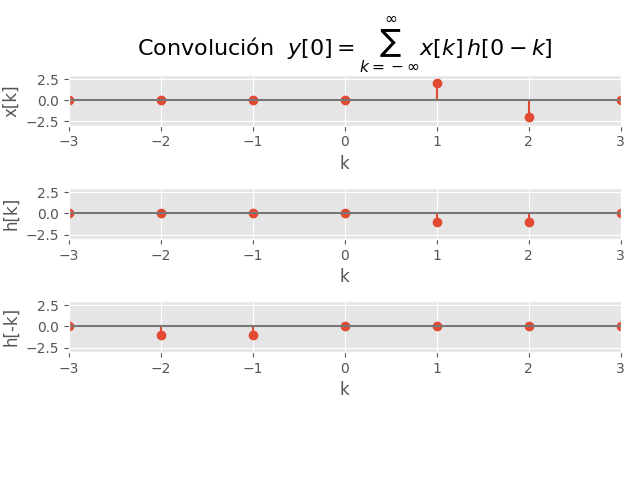
\includegraphics[width=6in]{./graphics/convejemp01-01.png}
    \caption{Se\~{n}ales $x[k]$, $h[k]$ y $h[-k]$.}
    \label{convejemp0101eps}
\end{figure}

\begin{figure}
	\centering
	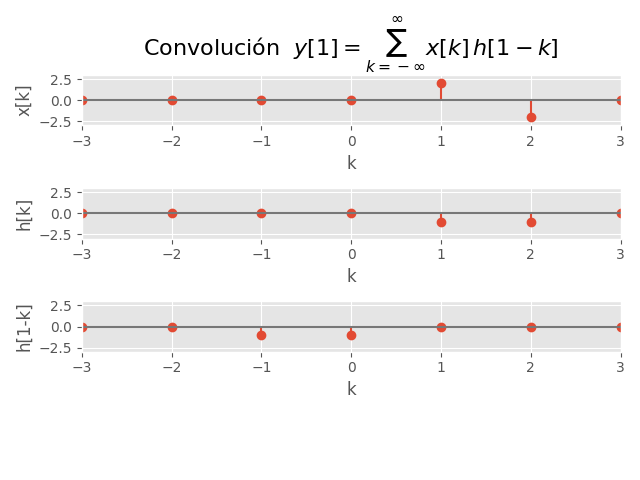
\includegraphics[width=6in]{./graphics/convejemp01-02.png}
    \caption{Se\~{n}ales $x[k]$, $h[k]$ y $h[1-k]$.}
	\label{convejemp0102eps}
\end{figure}

\begin{figure}
	\centering
	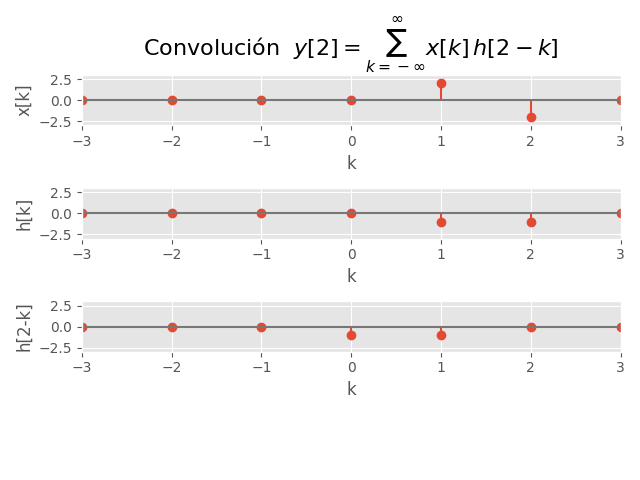
\includegraphics[width=6in]{./graphics/convejemp01-03.png}
    \caption{Se\~{n}ales $x[k]$, $h[k]$ y $h[2-k]$.}
	\label{convejemp0103eps}
\end{figure}

\begin{figure}
	\centering
	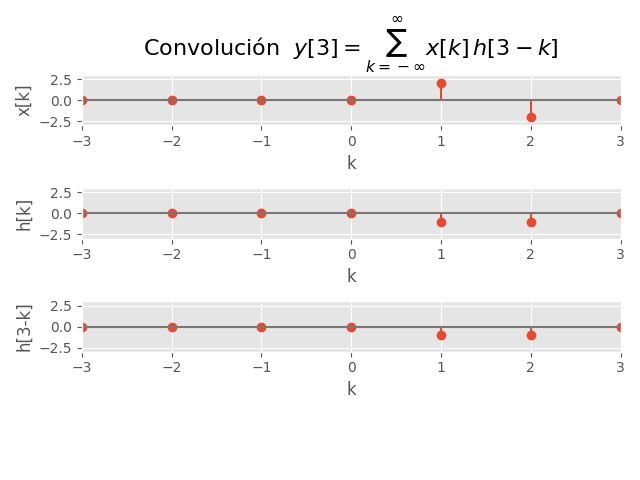
\includegraphics[width=6in]{./graphics/convejemp01-04.png}
    \caption{Se\~{n}ales $x[k]$, $h[k]$ y $h[3-k]$.}
	\label{convejemp0104eps}
\end{figure}

\begin{figure}
	\centering
	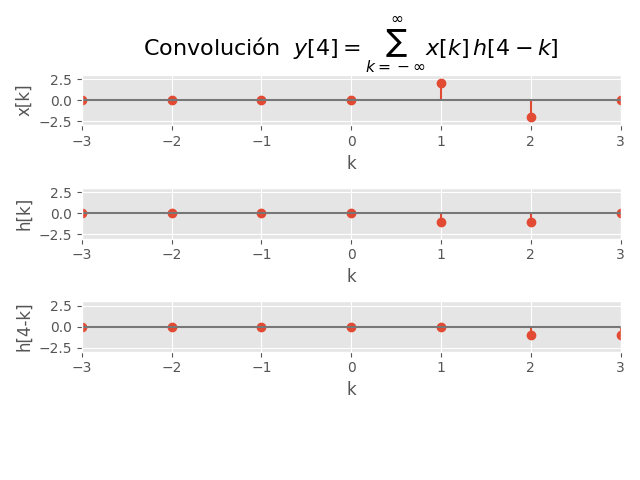
\includegraphics[width=6in]{./graphics/convejemp01-05.png}
    \caption{Se\~{n}ales $x[k]$, $h[k]$ y $h[4-k]$.}
	\label{convejemp0105eps}
\end{figure}

\begin{figure}
	\centering
	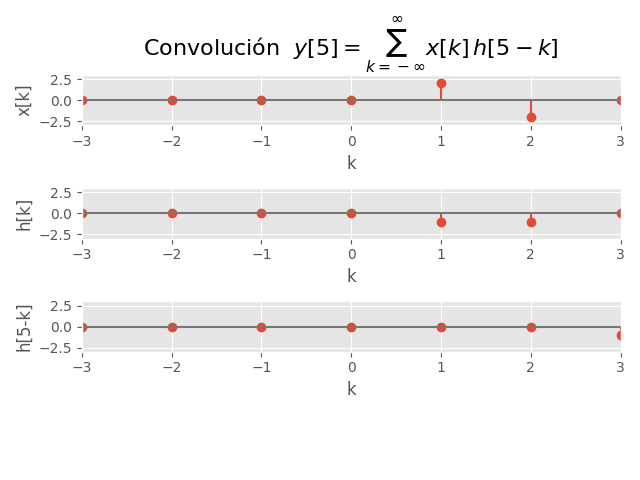
\includegraphics[width=6in]{./graphics/convejemp01-06.png}
    \caption{Se\~{n}ales $x[k]$, $h[k]$ y $h[5-k]$.}
	\label{convejemp0106eps}
\end{figure}


\subsection{Convoluci\'{o}n con un impulso}

Calculemos ahora la convoluci\'{o}n de las se\~{n}ales
\begin{eqnarray}
  x\left[ n\right] &=& \left( \frac{99}{100}\right) ^nu\left[ n\right] , \\
  h\left[ n\right] &=& \delta \left[ n-1\right] .
\end{eqnarray}

\subsubsection{Forma gr\'{a}fica}

\begin{enumerate}
\item Dibujemos las se\~{n}ales $x[k]$, $h[k]$ y $h[-k]$.
        
\item Dibujemos $h[n-k]$ para distintos valores de $n$, junto con
  $x[k]$. Ver (\ref{convejemp0201eps}).
        
\item Dibujemos el producto $z[n,k] = x[k] \, h[n-k]$.
        
\item Calculemos $\sum_{k}z[n,k]$ para obtener $y[n]$.
\end{enumerate}

\begin{figure}
	\centering
	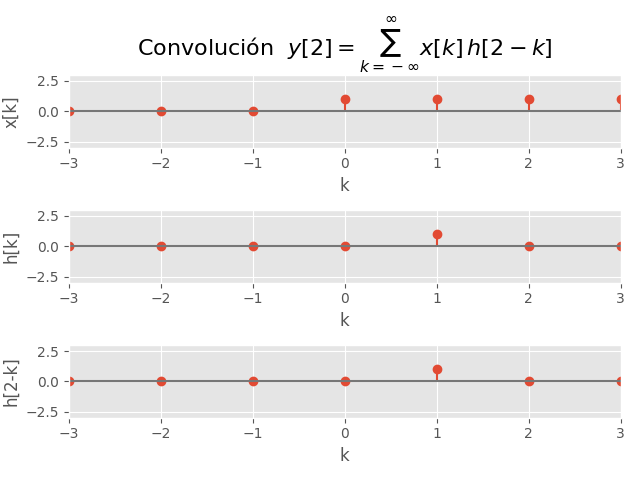
\includegraphics[width=6in]{./graphics/convejemp02-01.png}
    \caption{Se\~{n}ales $x[k]$, $h[k]$ y $h[2-k]$.}
	\label{convejemp0201eps}
\end{figure}

\subsubsection{Forma anal\'{\i}tica}

\begin{enumerate}
\item Seg\'{u}n la Ec. (\ref{convo}), tenemos
  \begin{equation}
    y\left[ n\right] =
    \sum_{k=-\infty }^{\infty }\left( \frac{99}{100}\right) ^{k}u \left[ k\right] \delta \left[ n-1-k\right].
  \end{equation}

\item Dado que dentro de la sumatoria aparece un escal\'{o}n unitario,
  podemos eliminarlo modificando adecuadamente el l\'{\i}mite inferior
  del \'{\i}ndice $k$.  Además, dado que la entrada contiene un factor escalón $u[n]$, la salida también tiene un factor similar. Entonces, 
  como $u[k] = 0$ para $k < 0$, el l\'{\i}mite
  inferior es $k = 0$, y además la sumatoria queda multiplicada por $u[n]$
  \begin{equation}
    y\left[ n\right] =\left(\sum_{k=0}^{\infty }\left( \frac{99}{100}\right) ^{k}\delta \left[ n-1-k\right]\right) \times u[n]. \label{ejeconvimpulso.0}
  \end{equation}

\item Observe que el \'{\i}ndice del impulso es $n - 1 - k$, y que por
  lo tanto est\'{a} ubicado en $k = n - 1$. Entonces
  \begin{equation}
    \sum_{k=0}^{\infty}\left( \frac{99}{100}\right) ^{k}\delta \left[ n-1-k\right] = 
    \left( \frac{99}{100}\right) ^{n-1}\delta \left[0\right] =
    \left( \frac{99}{100}\right) ^{n-1}
     \label{ejeconvimpulso}
  \end{equation}

\item Reemplazando (\ref{ejeconvimpulso}) en (\ref{ejeconvimpulso.0}), obtenemos
  \begin{equation}
  	y[n] = 
    \left( \frac{99}{100}\right) ^{n-1}
     \times u[n] .
  \end{equation}

\item En general, consideremos una respuesta al impulso
  \begin{equation}
    h\left[ n\right] = \delta \left[ n-n_{0}\right] .
  \end{equation}
  y calculemos su convoluci\'{o}n para una entrada gen\'{e}rica
  $x[n]$.

\item Seg\'{u}n la Ec. (\ref{convo}), tenemos
  \begin{equation}
    y\left[ n\right] =\sum_{k=-\infty }^{\infty } x[k] \, \delta \left[ n-n_{0}-k\right] ,
  \end{equation}

\item Observe que el \'{\i}ndice del impulso es $n - n_{0} - k$, y que
  por lo tanto est\'{a} ubicado en $k = n - n_{0}$. Entonces
  \begin{equation}
    x[k] \, \delta \left[ n-n_{0}-k\right] = x[n-n_{0}] \, \delta \left[0\right] = 
    x[n-n_{0}].
  \end{equation}

\item Considerando la sumatoria, obtenemos
  \begin{equation}
    \sum_{k=-\infty}^{\infty }x[n-n_{0}]\delta \left[ n-n_{0}-k\right] = 
    x[n-n_{0}] .
  \end{equation}

\item Dado que
  \begin{equation}
    u[n-n_{0}] = \left( \sum_{k=-\infty}^{\infty } \delta \left[ n-n_{0}-k\right] \right)
  \end{equation}
  la salida $y[n]$ es
  \begin{equation}
    y\left[ n\right] = x[n-n_{0}] \, u[n-n_{0}].
  \end{equation}
\end{enumerate}

\subsection{Convoluci\'{o}n de una se\~{n}al con una ventana
  rectangular}

Calculemos la convoluci\'{o}n de las se\~{n}ales
\begin{eqnarray}
  x\left[ n\right] &=&\left( \frac{1}{2}\right) ^nu\left[ n\right] ,                                      \\
  h\left[ n\right] &=&u\left[ n\right] -u\left[ n-2\right] =
  \delta \left[ n \right] +\delta \left[ n-1\right] ,
\end{eqnarray}

\subsubsection{Forma gr\'{a}fica}

\begin{enumerate}
\item Dibujemos las se\~{n}ales $x[k]$, $h[k]$ y $h[-k]$.
        
\item Dibujemos $h[n-k]$ para distintos valores de $n$, junto con
  $x[k]$.
        
\item Dibujemos el producto $z[n,k] = x[k] h[n-k]$.
        
\item Calculemos $\sum_{k}z[n,k]$ para obtener $y[n]$.
\end{enumerate}

\subsubsection{Forma anal\'{\i}tica}

% rehacer figura convo

\begin{enumerate}
\item Seg\'{u}n la Ec. (\ref{convo}), tenemos
  \begin{equation}
    y\left[ n\right] =
    \sum_{k=-\infty }^{\infty }\left( \frac{1}{2}\right) ^{k} \,
    u\left[ k\right] \, h\left[ n-k\right].
  \end{equation}

\item Ajustamos los \'{\i}ndices de la sumatoria porque la ventana
  rectangular es nula para $k < 0$
  \begin{equation}
    y\left[ n\right] =
    \sum_{k=0}^{\infty }\left( \frac{1}{2}\right) ^{k} \, h\left[n-k\right].
  \end{equation}
        
\item Expresamos a la ventana rectangular como una suma de impulsos
  desplazados en el tiempo
  \begin{equation}
    y\left[ n\right] =
    \sum_{k=0}^{\infty }
    \left( \frac{1}{2}\right) ^{k}\left(\delta \left[ n-k\right] +\delta \left[ n-1-k\right] \right).
  \end{equation}
        
\item Desdoblamos la convoluci\'{o}n en dos,
  \begin{eqnarray}
    \sum_{k=0}^{\infty }\left( \frac{1}{2}\right) ^{k} \, \delta \left[ n-k\right]
    &=&\left( \frac{1}{2}\right) ^n u[n], \\
    \sum_{k=0}^{\infty }\left( \frac{1}{2}\right) ^{k} \, \delta \left[ n-1-k\right]
    &=&\left( \frac{1}{2}\right) ^{n-1} u[n-1].
  \end{eqnarray}
        
\item El resultado final es
  \begin{equation}
    y\left[ n\right] =\left( \frac{1}{2}\right)^n \, u[n] +\left(
      \frac{1}{2}\right)^{n-1} \, u[n-1].
  \end{equation}
\end{enumerate}

\subsection{Convoluci\'{o}n de se\~{n}ales infinitas}

Considere una entrada $x\left[ n\right] $ y una respuesta al impulso
unitario dadas por
\begin{eqnarray}
  x\left[ n\right] &=&\alpha ^nu\left[ n\right] , \\
  h\left[ n\right] &=&u\left[ n\right] ,
\end{eqnarray}
donde el valor absoluto de $\alpha$ es menor que $1$, 
\begin{equation}
0< | \alpha | <1.
\end{equation}

\subsubsection{Forma gr\'{a}fica}

\begin{enumerate}
\item Dibujemos las se\~{n}ales $x[k]$, $h[k]$ y $h[-k]$.
        
\item Dibujemos $h[n-k]$ para distintos valores de $n$, junto con
  $x[k]$.
        
\item Dibujemos el producto $z[n,k] = x[k] \, h[n-k]$.
        
\item Calculemos $\sum_{k} z[n,k]$ para obtener una aproximaci\'{o}n de
  $y[n]$
\end{enumerate}

\subsubsection{Forma anal\'{\i}tica}

\begin{enumerate}
\item Seg\'{u}n la Ec. (\ref{convo}), tenemos
  \begin{equation}
    \alpha^{k} u[k] u[n-k] =
    \left\{ \begin{array}{ll}
        \alpha ^{k}, & 0\leq k\leq n, \\ 
        0, & \left( k<0\right) \vee \left( k>n\right)
      \end{array} \right.             \label{convinf}
  \end{equation}

\item Para poder realizar esta sumatoria, debemos recordar sucesiones
  geométricas.  Definamos la suma parcial
  \begin{equation}
    S_{n}=    \sum_{k=0}^n\alpha ^{k},
  \end{equation}
  y multipliquemos por $a$ para obtener
  \begin{equation}
    \alpha \, S_{n}=   \sum_{k=0}^n\alpha ^{k+1}.
  \end{equation}
  Entonces podemos escribir
  \begin{equation}
    S_{n}-\alpha \, S_{n}= \left( \sum_{k=0}^n\alpha ^{k}\right) - \left( \sum_{k=0}^n\alpha ^{k+1}\right)
  \end{equation}
  y simplificando
  \begin{equation}
    S_n- \alpha \, S_n=\alpha^{0}-\alpha^{n+1}.
  \end{equation}
  Podemos despejar entonces
  \begin{equation}
    S_n=\frac{\alpha^{0}-\alpha^{n+1}}{1-\alpha}=\frac{1-\alpha^{n+1}}{1-\alpha}.    \label{sumageo}
  \end{equation}

\item Aplicamos la Ec. (\ref{sumageo}) a la Ec. (\ref{convinf})
  \begin{equation}
    \sum_{k=0}^n\alpha ^{k}=\frac{1-\alpha ^{n+1}}{1-\alpha }.      \label{sumaserie}
  \end{equation}
  Por lo tanto, la respuesta es
  \begin{equation}
    y\left[ n\right] =\left( \frac{1-\alpha ^{n+1}}{1-\alpha }\right) u\left(n\right) .
  \end{equation}
\end{enumerate}

\subsection{Convoluci\'{o}n de una se\~{n}al consigo misma}

Vamos a calcular la convolución de una señal consigo misma, definiendo
\begin{eqnarray}
  x\left[ n\right] =\left( \frac{8}{10}\right)^n u\left[ n\right] ,       \\
  h\left[ n\right] =\left( \frac{8}{10}\right)^n u\left[ n\right] .
\end{eqnarray}

\subsubsection{Forma gr\'{a}fica}

\begin{enumerate}
\item Dibujemos las se\~{n}ales $x[k]$, $h[k]$ y $h[-k]$.
        
\item Dibujemos $h[n-k]$ para distintos valores de $n$, junto con
  $x[k]$.
        
\item Dibujemos el producto $z[n,k] = x[k] h[n-k]$.
        
\item Calculemos $\sum_{k}z[n,k]$ para obtener $y[n]$ en forma
  aproximada
\end{enumerate}

\subsubsection{Forma anal\'{\i}tica}

\begin{enumerate}
\item Seg\'{u}n la Ec. (\ref{convo}), tenemos
  \begin{equation}
    y\left[ n\right] =
    \sum_{k=-\infty }^{\infty }
    \left( \frac{8}{10}\right)^{k} u\left[ k\right] 
    \left( \frac{8}{10}\right)^{n-k} u\left[ n-k\right] ,
  \end{equation}

\item Podemos modificar los l\'{\i}mites de la sumatoria, pues $u[k] =
  $ para $k < 0$, y $u[n-k] = 0$ para $n - k < 0$
  \begin{equation}
    y\left[ n\right] = (\sum_{k=0}^{n }\left( \frac{8}{10}\right) ^{k+n-k}) \times u[n].
  \end{equation}
   Observe que si uno de los factores de la entrada es un escalón $u[n - n_{0}]$, la salida también tiene el mismo factor.
   
\item Extraemos de la sumatoria el factor com\'{u}n de todos los
  sumandos $(\frac{8}{10})^{n}$, que es independiente de $k$, y obtenemos
  \begin{equation}
    y\left[ n\right] = \left(\left( \frac{8}{10}\right) ^{n} \sum_{k=0}^{n} 1\right) \times u[n],
  \end{equation}

\item Finalmente resulta esto
  \begin{equation}
    y\left[ n\right] = \left( \frac{8}{10}\right) ^{n} \, \left(n+1
    \right) \, u[n].
  \end{equation}
  El factor $u[n]$ aparece porque la sumatoria cuyo resultado es $n +
  1$ tiene un l\'{\i}mite inferior $k = 0$, y por lo tanto la sumatoria es no nula sí y solo sí $n \geq 0$.
\end{enumerate}
